\begin{frame}{What is an Adversarial Example?}
  \onslide<+->{
    \begin{definition}
      \textit{\green{Adversarial Example}}: An input chosen/modified by an adversary that is almost indistinguishable from natural data but is (confidently) misclassified by the network.
    \end{definition}
  }

  \begin{columns}
    \begin{column}{0.23\textwidth}
      \onslide<+->{
        \begin{center}
          
\includegraphics{adv_panda}

          \textbf{\blue{Prediction}}
          \\
          \textbf{Panda}
          \\
          55.7\% Confidence~\cite{Goodfellow:2014}
        \end{center}
      }
    \end{column}
    \onslide<+->{
      \begin{column}{0.05\textwidth}
          \begin{center}
            +\vspace{1.6cm}
          \end{center}
      \end{column}
      \begin{column}{0.20\textwidth}
          \begin{center}
            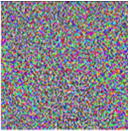
\includegraphics{adv_noise}

            \textbf{\blue{Prediction}}
            \\
            \textbf{Nematode}
            \\
            8.2\% Confidence
          \end{center}
      \end{column}
    }
    \onslide<+->{
      \begin{column}{0.05\textwidth}
          \begin{center}
            =\vspace{1.6cm}
          \end{center}
      \end{column}
      \begin{column}{0.20\textwidth}
          \begin{center}
            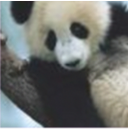
\includegraphics{adv_combined}
            \textbf{\blue{Prediction}}
            \\
            \textbf{Gibbon}
            \\
            99.3\% Confidence
          \end{center}
      \end{column}
    }
    \onslide<+->{
      \begin{column}{0.20\textwidth}
          \begin{center}
            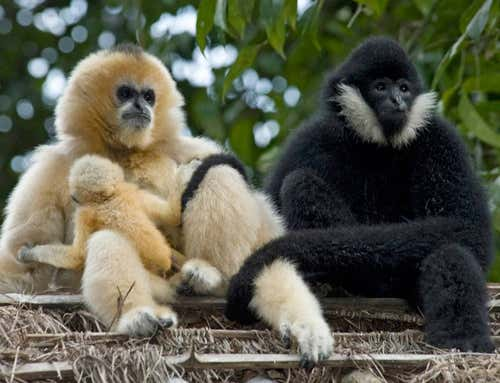
\includegraphics[scale=0.15]{gibbon}
            \textbf{\red{Actual}\\Gibbon}
          \end{center}
      \end{column}
    }
  \end{columns}

\end{frame}


\begin{frame}{Attack Paradigms}
  \madry\ study adversarial robustness under two different attack paradigms:
  \vfill
  \begin{enumerate}[<+->]
    \item \textbf{Black-Box}: Adversary has no direct access to target network
      \begin{itemize}[<+->]
        \setlength\itemsep{6pt}
        \item \red{Weaker} attack paradigm
        \item Adversary may have \textit{rough} information, e.g.,~model architecture \& training dataset
          \begin{itemize}
            \item \textit{Example}: Transfer attack
          \end{itemize}
        \item Generally \textit{one-shot} attacks
      \end{itemize}
    \vfill
    \item \textbf{White-Box}: Attacker has access to target network's parameter
      \begin{itemize}
        \setlength\itemsep{6pt}
        \item \green{Stronger} attack paradigm
        \item \textit{Examples}: PGD and FGSM (both discussed in this talk)
        \item Enables \textit{iterative} attacks, e.g.,~refined probing
      \end{itemize}
  \end{enumerate}
\end{frame}


\begin{frame}{$\ell_{p}$ Balls --- Norms First}
  For ${x \in \mathbb{d}}$, the $L_{p}$ norm is:

  \begin{equation}\label{eq:LpNorm}
    \norm{x}_{p} = \left( \sum_{i=1} x_{i}^{p}  \right)^{\frac{1}{p}}
  \end{equation}

  $L_{\infty}$ norm is a special a case:

  \begin{equation}\label{eq:LinftyNorm}
    \norm{x}_{\infty} = \sup_{i} \abs{x_i}
  \end{equation}

  \begin{center}
    \textbf{Note}: $\sup$ equals the $\max$ for a finite set
  \end{center}
\end{frame}

\begin{frame}{$\ell_{p}$ Balls --- Let's Visualize\ldots}
  \begin{definition}
    Given scalar ${\varepsilon > 0}$, the $\ell_{p}$ ball of a point ${x \in \mathbb{R}^{d}}$ is:

    \begin{equation}\label{eq:LpBall}
      \ell_{p}(x) = \setbuild{x + \delta}{\norm{\delta}_{p} \leq \varepsilon}\text{.}
    \end{equation}
  \end{definition}

  \onslide<+->{
    \begin{center}
      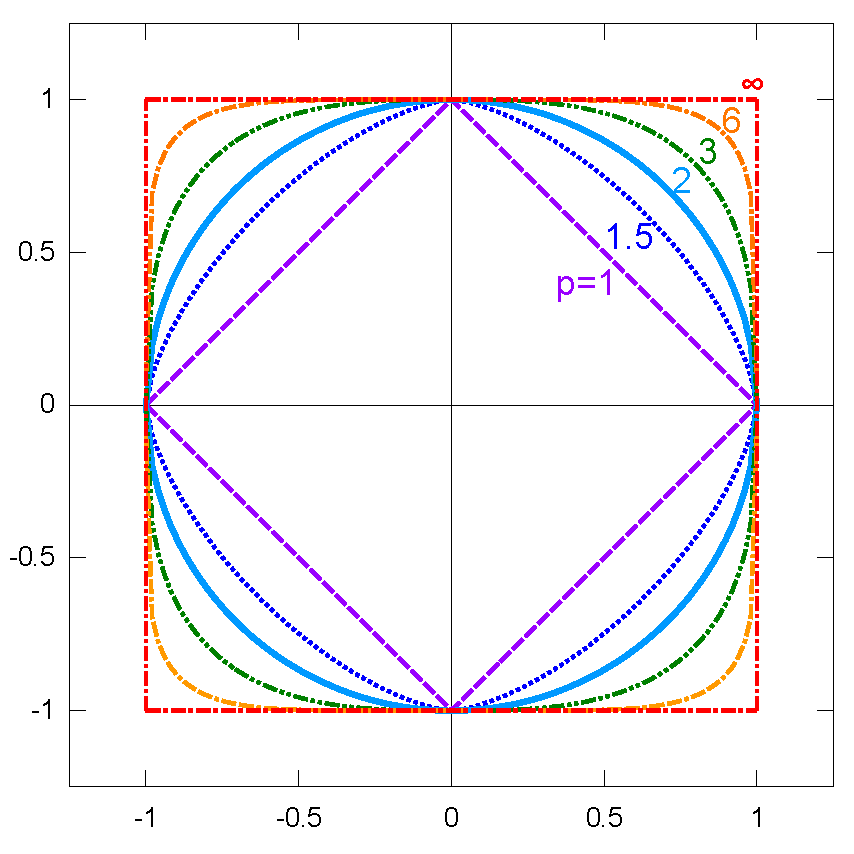
\includegraphics[scale=0.29]{img/lpballs.pdf} \cite{wiki:Lp_space}
    \end{center}
  }
\end{frame}
